% ||||||||||||||| <<<<< COMPILIEREN MIT pdflatex --shell-escape Dima-Hadoop-Vortrag.tex >>>>>> ||||||||||||||||||||||||||

\documentclass{beamer}

% ++++++++++++++++++++++++++++++++++++++++++++++++++++++++++++++++++ 
% +++ Theme ++++++++++++++++++++++++++++++++++++++++++++++++++++++++
% ++++++++++++++++++++++++++++++++++++++++++++++++++++++++++++++++++ 
\usetheme{dima}
\logo{
\includegraphics[width=1cm]{dimalogo.pdf}}

% ++++++++++++++++++++++++++++++++++++++++++++++++++++++++++++++++++ 
% +++ Positionierung und Beschriftung von Bildern ++++++++++++++++++
% ++++++++++++++++++++++++++++++++++++++++++++++++++++++++++++++++++ 
% enable eps graphic files
\usepackage[cleanup={log,aux,dvi,ps,pdf}]{auto-pst-pdf}
% enable absolute positioning on frames
\usepackage[absolute,overlay]{textpos}
% adjust the TPHorizModule and TPHorizModule units to the displayed mm grid Anzahl der horizontalen und vertikalen Linien des Beamer Grids
\TPGrid{13}{10}
% beschriftungen
\usepackage{overpic}
% grid for positioning \setbeamertemplate{background}[grid][step=1cm]


% ++++++++++++++++++++++++++++++++++++++++++++++++++++++++++++++++++ 
% +++ Encoding +++++++++++++++++++++++++++++++++++++++++++++++++++++
% ++++++++++++++++++++++++++++++++++++++++++++++++++++++++++++++++++ 
% verwende Vektorschriften, falls vorhanden
\usepackage[T1]{fontenc}

% Encodierung der Quelldatei latin1 = ISO 8859-1 ansinew = Windows applemac = Apple-Mac utf8 = UTF-8-Encoding
\usepackage[utf8]{inputenc}


% ++++++++++++++++++++++++++++++++++++++++++++++++++++++++++++++++++ 
% +++ Schriften ++++++++++++++++++++++++++++++++++++++++++++++++++++
% ++++++++++++++++++++++++++++++++++++++++++++++++++++++++++++++++++ 
% verwendete Schriften Doku:
% http://www.ctan.org/tex-archive/macros/latex/required/psnfss/psnfss2e.pdf
\usepackage{charter}
\usepackage[scaled=.92]{helvet}
\usepackage{courier}

% besseres Schriftbild Doku: http://www.ctan.org/tex-archive/macros/latex/contrib/microtype/microtype.pdf
\usepackage{microtype}


%++++++++++++++++++++++++++++++++++++++++++++++++++++++++++++++++++
%+++ Bilder +++++++++++++++++++++++++++++++++++++++++++++++++++++++
%++++++++++++++++++++++++++++++++++++++++++++++++++++++++++++++++++
% Für Floatobjekte
\usepackage{float}
% \FloatBarrier - Ermöglicht das forcierte Setzen von ausstehenden Floats. section macht vor jede section eine barrier.
\usepackage[section]{placeins} 

% Paket um Grafiken einbetten zu können
\usepackage{graphicx}
\graphicspath{{images/}}
\usepackage{subfigure}

% Zeilenumbruch bei Bildbeschreibungen.
%\setcapindent{1em}


%++++++++++++++++++++++++++++++++++++++++++++++++++++++++++++++++++
%+++ Sprache ++++++++++++++++++++++++++++++++++++++++++++++++++++++
%++++++++++++++++++++++++++++++++++++++++++++++++++++++++++++++++++
% neue Deutsche Rechtschreibung: Trennregeln!
\usepackage[english,german,ngerman]{babel}


%++++++++++++++++++++++++++++++++++++++++++++++++++++++++++++++++++
%+++ Literatur ++++++++++++++++++++++++++++++++++++++++++++++++++++
%++++++++++++++++++++++++++++++++++++++++++++++++++++++++++++++++++
\usepackage[german]{babelbib}


%++++++++++++++++++++++++++++++++++++++++++++++++++++++++++++++++++
%+++ Verlinkung +++++++++++++++++++++++++++++++++++++++++++++++++++
%++++++++++++++++++++++++++++++++++++++++++++++++++++++++++++++++++
% Doku: http://www.ctan.org/tex-archive/macros/latex/contrib/hyperref/hyperref.pdf
%\usepackage[%
%pdfauthor={Erik Nijkamp and Alexander Alexandrov and Jan Marc Hoffmann},
%colorlinks, % verwende farbige Links
%linkcolor=blue, % Linkfarbe ist blau
%bookmarks, % erstelle Bookmarks der Links
%bookmarksopenlevel=1, % nur bis level 1 öffnen
%bookmarksopen, % Bookmarks werden beim öffnen des Dokumentes ebenfalls geöffnet
%urlcolor=blue, % Hyperlinks sind blau 
%citecolor=blue, % Cite Links sind blau
%bookmarksnumbered, % Bookmarks sind nummeriert
%final % Endversion 
%]{hyperref}

% fokusiert captions korrekt
%\usepackage[all]{hypcap}

\usepackage{listings}
% Listings Konfiguration
\lstset{language=Java, commentstyle=\color[RGB]{63,127,95}\ttfamily,
  keywordstyle=\color[RGB]{127,0,85}\bfseries,
  stringstyle=\color[RGB]{42,0,255}\ttfamily, showstringspaces=false,
  tabsize=2,
  % numbers=left,
  numberstyle=\tiny, numberblanklines=true, stepnumber=1,
  numbersep=5pt, xleftmargin=5pt,
  emphstyle=\color[RGB]{0,0,192}\texttt, breaklines=true,
  breakautoindent=true,
  % basicstyle=\tiny,
  extendedchars=true,
  % frame=shadowbox, rulesepcolor=\color{gray}
  %morekeywords={team,playedBy,as,when,after,before,base,within,replace,result,activate,deactivate}, %Erweiterung fuer Object Teams
  backgroundcolor=\color{white}, 
  framexleftmargin=2mm, 
  frame=shadowbox, 
  rulesepcolor=\color{lightgray}
}

% %%%%%%%%%%%%%%%%%%%%%%%%%%%%%%%%%%%%%%%%%%%%%%%%%%%%%%%% 
% Informationen zum Dokument
% %%%%%%%%%%%%%%%%%%%%%%%%%%%%%%%%%%%%%%%%%%%%%%%%%%%%%%%%

\author{\textcolor{gray}{Projektleiter:} Foo Bar\\ \textcolor{gray}{Team:}
Autor 1, Autor 2}
\title{Projekt -- Ein Query-Optimizer für Cloudsysteme}
%s\subtitle{lll}
\institute{Datenbanksysteme und Informationsmanagement \\
Technische Universität Berlin \\[0.5cm]

\includegraphics[width=1.8cm]{tulogo}}
%\university{ss}
\date{\today}



% %%%%%%%%%%%%%%%%%%%%%%%%%%%%%%%%%%%%%%%%%%%%%%%%%%%%%%%% 
% Dokument 
% %%%%%%%%%%%%%%%%%%%%%%%%%%%%%%%%%%%%%%%%%%%%%%%%%%%%%%%%%

\begin{document}

% --------------------------------------------------------
\begin{frame}
\maketitle
\end{frame}
%--------------------------------------------------------

%--------------------------------------------------------
\begin{frame}
\frametitle{Agenda}
\tableofcontents
\end{frame}
%--------------------------------------------------------

% %%%%%%%%%%%%%%%%%%%%%%%%%%%%%%%%%%%%%%%%%%%%%%%%%%%%%%%% 
% Folien 
% %%%%%%%%%%%%%%%%%%%%%%%%%%%%%%%%%%%%%%%%%%%%%%%%%%%%%%%%%

\section{Projektziele}

% --------------------------------------------------------------------------------------------------------------
\begin{frame}
\frametitle{Projektziele}
Effiziente Implementierung relationaler Joins im Hadoop-Framework
\hspace{8pt}
\begin{itemize}
  \item 2 Verfahren
  \begin{itemize}
    \item Realisierung ohne Veränderung des Hadoop-Frameworks
    \item Erweiterung des Hadoop-Frameworks um einen
    Merge-Operator
  \end{itemize}
  \item Tests der Verfahren gegeneinander
\end{itemize}
\end{frame}
% --------------------------------------------------------------------------------------------------------------

\section{Untersuchte Joinverfahren}

% ------------------------------------------------------------------------------
\begin{frame}
\frametitle{Agenda}
\tableofcontents[currentsection]
\end{frame}
% ------------------------------------------------------------------------------

% ------------------------------------------------------------------------------
\begin{frame}[fragile]
\frametitle{Repartition Join}
\begin{itemize}
  \item Equi-Join über 2 Relationen
  \item Mapper: wird jedes Tupel einmal weitergegeben oder ausgefiltert
  \item Partitioner: Modulo-Division des Schlüssel-HashWerts
\end{itemize}

\scriptsize{
\lstset{framexleftmargin=5mm, frame=shadowbox, rulesepcolor=\color{lightgray}}
\begin{lstlisting}
public void map(...) throws IOException 
{
    RelationTuple tuple = new RelationTuple(value);
    ...
    if (!filter.eval(tuple)) output.collect(outputKey, tuple);
}
\end{lstlisting}

\lstset{framexleftmargin=5mm, frame=shadowbox, rulesepcolor=\color{lightgray}}
\begin{lstlisting}
public int getPartition(RepartitionKey k, RelationTuple v, int ptns) 
{
    return Math.abs(k.getKey().hashCode() % ptns);
}
\end{lstlisting}
}
\end{frame}
% ------------------------------------------------------------------------------

% ------------------------------------------------------------------------------
\begin{frame}[fragile]
\frametitle{Repartition Join}
\begin{itemize}
  \item Sort:
  \begin{itemize} 
    \item primär nach Key 
    \item sekundär nach Relation ($L$ Relation kommt zuerst)
  \end{itemize}
  \item Reduce:
  \begin{itemize}
    \item alle $L$-Tupel zum aktuellen Schlüssel sammeln
    \item mit allen passenden $R$-Tupel kombinieren (kommen gleich danach)
  \end{itemize}
\end{itemize}
\end{frame}
% ------------------------------------------------------------------------------

% ------------------------------------------------------------------------------
\begin{frame}
\frametitle{TPCH Schema}
\begin{center}
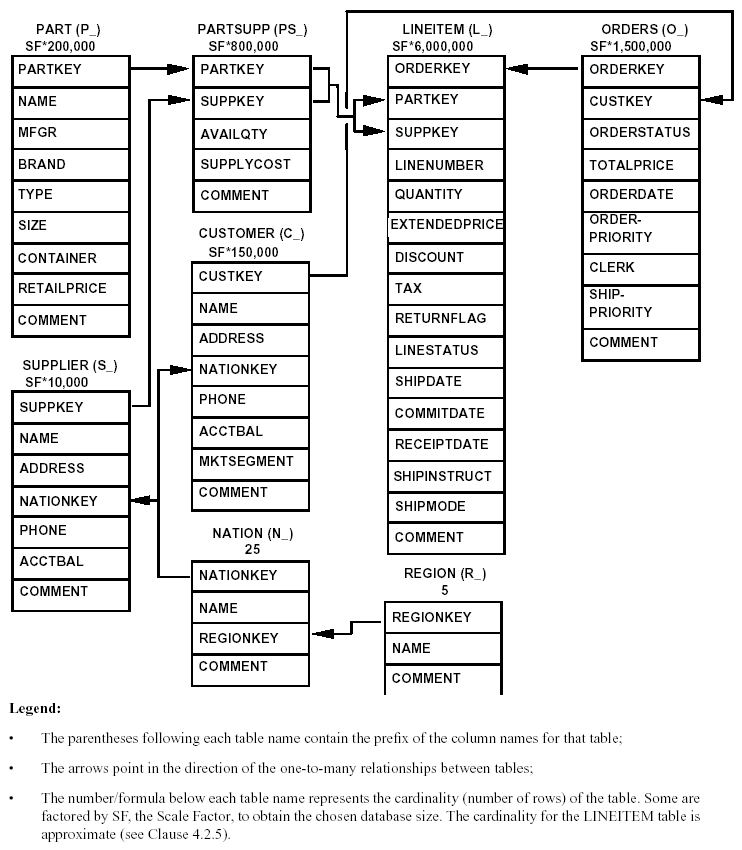
\includegraphics[width=.9\linewidth]{tpch-schema}
\end{center}
\end{frame}
% ------------------------------------------------------------------------------


%--------------------------------------------------------
\begin{frame}
\frametitle{Vielen Dank für Ihre Aufmerksamkeit}
\begin{center}
{\LARGE Fragen?}
\end{center}
\bibliographystyle{babalpha}
\bibliography{bib/references}
\nocite{*}
\end{frame}
%--------------------------------------------------------

\end{document}
